\documentclass{beamer}
\usepackage{xspace}
\usepackage{quiver}
\usepackage{xeCJK}
%\usepackage{subfig}
\usepackage{amsmath,extarrows}
\usepackage{amssymb}
%\usepackage{color}
\usepackage{fontspec}
\usepackage{minted}
\usepackage{mathtools}
\usepackage{hyperref}
\usepackage{mathpartir}
\input{Style/preamble.tex}
\usepackage{Style/listproc}
\usepackage{Style/ottalt}
\inputott[rp]{Data/report.ott}
\inputott[dd]{Data/tigrisd}
\renewottcommands[rp]

\newmintinline[lean]{lean4}{bgcolor=white}
\newminted[leancode]{lean4}{fontsize=\footnotesize}
\newmintinline[ocaml]{ocaml}{bgcolor=white}
\newminted[ocamlcode]{ocaml}{fontsize=\footnotesize}
\setmonofont{Victor Mono}[Scale=.85]
\usetheme{CambridgeUS}
\usecolortheme{dove}
\usefonttheme{serif}
\makeatletter
\renewcommand*\verbatim@nolig@list{}
\makeatother

\newcommand\blfootnote[1]{%
  \begingroup
  \renewcommand\thefootnote{}\footnote{#1}%
  \addtocounter{footnote}{-1}%
  \endgroup
}

\DeclareMathOperator{\op}{\mathsf{op}}

\title{TinyTheorem}
\subtitle{一个依值类型的编程语言暨定理证明器原型\\A prototype for a dependently-typed programming language\\ with theorem proving}
\date{\today}
\author{Zhenming Gao\inst{1}}

\institute[SCNU]{
  \inst{1}%
  School of Artificial Intelligence\\
  South China Normal University
}

\logo{
\includegraphics[height=.8cm]{Style/Figures/SCNUBadge}}

\begin{document}
\frame{\titlepage}
\section{intro}
\subsection{Premise}
\begin{frame}\frametitle{Challenge \& Motivation}
  Recently:
  \begin{itemize}
    \item<1-> LLM \& AI4MATH attracted mathematicians such as Terence Tao, circa 2024 $\to$ PLT, TT, Cat
    \item<2-> React \& Vue: Functional programming on the frontend,
      TypeScript's gradual type system $\to$ Advanced Functional Programming, PLT
  \end{itemize}
  \onslide<3->{
    \begin{block}{Challenge: theory-heavy}
      PL education and academic (functional) programming practices
    \end{block}
  }
  \onslide<4->{
    \begin{alertblock}{TinyTheorem}
      solid platform for teaching, experimentation, \& verification
    \end{alertblock}
  }
\end{frame}
\subsection{Overview}
\begin{frame}
  \frametitle{TinyTheorem\footnote{code available at \href{https://github.com/notch1p/tigris}{github.com/notch1p/tigris}\\ thesis at \href{https://github.com/notch1p/beng-thesis}{github.com/notch1p/beng-thesis}} = Tigris + Tigrisd}
  \begin{itemize}
    \item a language and toolchain prototype
    \item aims at industrial programming
      \begin{itemize}
        \item the \emph{Tigris} programming language
      \end{itemize}
    \item while simultaneously being theorem proving-oriented
      \begin{itemize}
        \item the \emph{Tigrisd} theorem prover
      \end{itemize}
  \end{itemize}
  \begin{alertblock}{Keywords}
    programming language, type theory, theorem prover, compiler
  \end{alertblock}
\end{frame}
\section{Tigris}
\subsection{Overview}
\begin{frame}
  \frametitle{Tigris: A Functional Pure Language}
  \begin{itemize}
    \item<1-> \emph{pure}: functions in the mathematical sense
    \item<1-> \underline{proper} functional language: extended \elambdacalc as \emph{core calculus},
      expressive type system based on Hindley-Milner + Typeclasses
    \item<2-> concise \& unified syntax in CAML tradition + heavily influenced by Lean \& Haskell with
      support for custom operators
    \item<3-> using \Lambdair and compiles to Common Lisp (SBCL), enabling FFI
    \item<3-> accessible via compiler CLI frontend \& an experimental incremental interpreter
  \end{itemize}
\end{frame}
\subsection{Syntax}
\begin{frame}[fragile]
  \frametitle{A Glimpse of Tigris}
  \begin{columns}
    \begin{column}{.5\textwidth}
      Simple \texttt{List} (linked list) impl
      \begin{ocamlcode}
type List a = Nil | Cons a (List a)
infixr 67 "::" => Cons
let rec map f
  | Nil => Nil
  | x :: xs => f x :: map f xs
let rec foldl f init
  | Nil => init
  | x :: xs => foldl f (f init x) xs
let hd (x :: _) = x and tl (_ :: xs) = xs
      \end{ocamlcode}
  The \texttt{Eq} Typeclass
  \begin{leancode}
class Eq a = {eq : a -> a -> Bool}
instance Eq Int = {eq x y = __eqInt x y}
instance ∀a [Eq a], Eq (Option a) =
  { eq
    | None, None => true
    | Some a, Some b => a = b
    | _, _ => false }
  \end{leancode}
    \end{column}
    \begin{column}{.5\textwidth}
      Curried \& Higher-order fun(app)
      \begin{ocamlcode}
type Boxed = Boxed (Int -> Int -> Int)
let bAdd = Boxed (_ + _)
let unwrap (Boxed f) = f
let main =
  let (Boxed bAdd') = bAdd in
  ( unwrap bAdd 20 20
  , bAdd' 30 30)
      \end{ocamlcode}
      Operator-extended Let-binding
      \begin{ocamlcode}
type Option a = None | Some a
infixl 70 "<+>"
let rec xs <+> ys =
  match xs, ys with
  | x :: xs, y :: ys => 
    x + y + xs <+> ys
  | Nil, Nil => 0
  | _, _ => 0
let Some x <*> Some y = Some $ x * y
      \end{ocamlcode}
    \end{column}
  \end{columns}
\end{frame}
\subsection{Implementation Notes}
\begin{frame}
  \begin{itemize}
    \item<1-> Parsing: monadic parser combinator + Pratt parsing
    \item<2-> Type System: Extended HM with typeclass +
    strict higher-kinded types (HKT) \& arbitrary-ranked types\footnote{only appear inside constructors.},
    guarded by \emph{skolemization} and careful design, also does System F elaboration
    \item<3-> IR, CPS, Codegen pipeline: Lambda IR $\xrightarrow{\text{Opt}}$ Closure Conversion $\xrightarrow{\text{Opt}}$ CPS Transformation $\to$ Common Lisp
  \end{itemize}
  \onslide<2->{\[
  \inferrule[I-Ascribe-Poly]
  {\Gamma \vdash e \Rightarrow \rpnt{ty}_e\,;\, C_e
    \sigma = \forall \bar{\alpha}.\, \bar{\pi} \Rightarrow \rpnt{ty} \\
    \bar{\beta} = \fresh^{|\bar{\alpha}|} \\
    \theta = [\bar{\alpha} \mapsto \bar{\beta}] \\
    \rpnt{ty}_{\mathsf{inst}} = \theta(\rpnt{ty}) \\
    %%
    C_0 = \text{current constraints} \\
    (\theta', \_) = \solvesf(C_0, \rpnt{ty}_e \sim \rpnt{ty}_{\mathsf{inst}}) \\
    %%
    \rigid = \text{current rigid set} \\
    \forall (\alpha \mapsto \rpnt{ty}') \in \theta'.\;
    \alpha \in \rigid \implies \rpnt{ty}' = \alpha \\
    %%
    \rpnt{ty}_{\mathsf{sk}} = \skolem(\sigma) \\
    \text{add constraints for}\ \bar{\pi}
  }
  {\Gamma \vdash (e : \sigma) \Rightarrow \rpnt{ty}_{\mathsf{inst}}\,;\,
  C_e, \rpnt{ty}_e \sim \rpnt{ty}_{\mathsf{inst}}}
  \]}
\end{frame}
\subsection{Type System}
\begin{frame}\frametitle{Core Calculus}
The type checker runs on:
{\small\nonterms{expr}}
\end{frame}
\begin{frame}
Reconstructing types given by:
{\small\nonterms{typeexpr}}
\begin{itemize}
  \item Tigris implements a constraint-solving typechecker, generating constraints
  throughout the inference process, solving through unification afterwards.
\end{itemize}
\end{frame}
\subsection{More examples: HKT and Typeclasses}
\begin{frame}[fragile]
\begin{columns}
  \begin{column}{.5\textwidth}
    \texttt{Monad} design pattern
    \begin{minted}{lean4}
class Monad (m : 1) =
  { pure : forall a, a -> m a
  , bind : ∀a b, m a -> (a -> m b) 
                     -> m b}
infixr 90 ">>=" => bind

instance Monad Option =
  { pure x = Some x
  , bind
    | None, _ => None
    | Some x, f => f x}

let main : Option Int =
  pure 20 >>= fun x =>
    None >>= fun y =>
      pure 30 >>= fun z =>
        pure $ x + y + z
    \end{minted}
  \end{column}
  \begin{column}{.5\textwidth}
    \texttt{Functor} design pattern
    \begin{minted}{lean4}
class Functor (m : 1) = 
  {map : ∀a b, (a -> b) -> m a 
                        -> m b}
infixr 100 " <$> " => map

instance Functor List = 
  { map f x =
      let rec go 
        | Nil => Nil
        | x :: xs => 
          f x :: go xs
      in go f x}

let main =
  let k x _ = x in
  ( (2 + _) <$> Some 1
  , k "0" <$> 1 :: 2 :: Nil)
    \end{minted}
  \end{column}
\end{columns}
\end{frame}
\subsection{More examples: Mutual Recursion}
\begin{frame}[fragile]
\begin{minted}{ocaml}
mutual
  type Tree a = Empty | Node a (Forest a)
  type Forest a = Nil | Cons (Tree a) (Forest a)
;;

let rec countTree
  | Empty    => 0 
  | Node _ f => 1 + countForest f
and countForest
  | Nil      => 0 
  | Cons t f => countTree t + countForest f

(* f $ x = f x, lowest precedence, right associative  *)
let 5 = countTree
      $ Node 1 
      $ Cons (Node 2 $ Cons (Node 5 Nil) Nil)
      $ Cons (Node 3 $ Cons (Node 4 Nil) Nil)
      $ Cons Empty Nil
\end{minted}
\end{frame}
\subsection{Continuation Monad}
\begin{frame}[fragile]
\begin{minted}{ocaml}
type Cont a r = Cont ((a -> r) -> r) ;; infixr 90 ">>="

let return x = Cont fun k => k x
let run (Cont kf) k = kf k

let Cont kf >>= f = Cont fun k =>
  kf $ fun a =>
    let (Cont k') = f a 
    in k' k

let callcc f = Cont fun k =>
  let (Cont kf) = f $ fun a => Cont fun _ => k a 
  in kf k

let f = callcc fun k => return 0 >>= fun _ => k 42

let main = run f (fun x => x)
\end{minted}
\end{frame}
\section{Tigrisd}
\subsection{Overview}
\begin{frame}
  \frametitle{Tigrisd: A dependently-typed theorem prover}
  \centering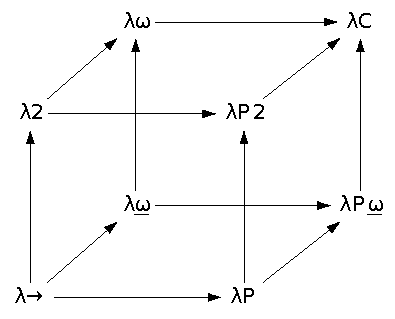
\includegraphics[scale=.8]{assets/Lambda_Cube.pdf}
  \begin{itemize}
    \item types may depend on values, types $\in$ terms
    \item type theory (system) much more expressive than Tigris, intuitionistic (Martin-Löf).
    \begin{itemize}
      \item Somewhere between $\lambda_{\Pi 2}$ and $\lambda_{\underline{\omega}}$
      \item \textbf{bare minimum}: dependent type theory + inductive constructions

    \end{itemize}
    \item parser + typechecker/evaluator implementation only
  \end{itemize}
\end{frame}
\subsection{Preliminary}
\begin{frame}\frametitle{Curry-Howard Isomorphism \& Computational Trilogy}
\begin{itemize}
  \item ``different perspectives on a single underlying phenomenon at the foundations of mathematics'' (per nLab)
\end{itemize}
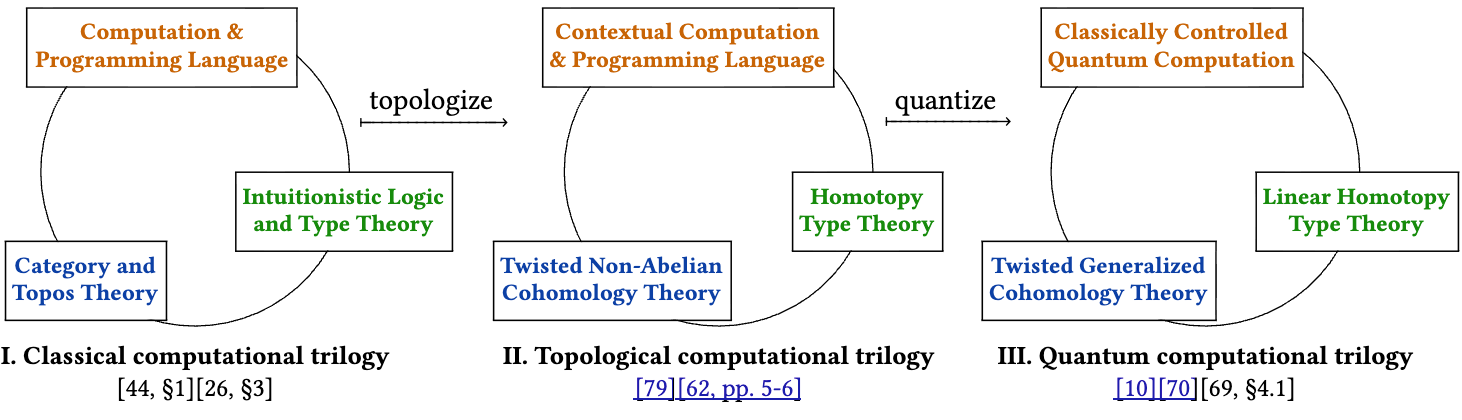
\includegraphics[scale=.48]{assets/trilogy.png}\footnote{Sati, Hisham, and Urs Schreiber. "Topological quantum programming in TED-K." arXiv preprint arXiv:2209.08331 (2022)}

\begin{alertblock}{C-H Correspondence}
Propositions as types; Proofs as terms.
\end{alertblock}
\end{frame}
\renewottcommands[dd]
\begin{frame}
% https://q.uiver.app/#q=WzAsMjEsWzAsMSwieFxcbWFwc3RvIHgiXSxbMSwxLCI6Il0sWzIsMSwiXFxmb3JhbGwgXFxhbHBoYS5cXDtcXGFscGhhXFx0b1xcYWxwaGEiXSxbMCwzLCJ4IDogXFxhbHBoYVxcbWFwc3RvIChoIDogXFxiZXRhXFwgeCkiXSxbMCwyLCJ4XFxtYXBzdG8geSJdLFsxLDIsIjoiXSxbMiwyLCJcXGZvcmFsbCBcXGFscGhhLlxcO1xcYWxwaGFcXHRvXFxiZXRhIl0sWzEsMywiOiJdLFswLDQsIlxcbGFuZ2xlIGEgOiBcXGFscGhhLCBoOlxcYmV0YVxcIGFcXHJhbmdsZSJdLFsxLDQsIjoiXSxbMiw0LCJcXGV4aXN0cyB4IDogXFxhbHBoYS5cXDtcXGJldGFcXCB4IDo9IFxcU2lnbWFfe3ggOiBcXGFscGhhfVxcIFxcYmV0YVxcIHgiXSxbMCw1LCJcXG5lZyBwIl0sWzEsNSwiXFxlcXVpdiJdLFsyLDUsInBcXHRvXFxtYXRoc2Z7RmFsc2V9Il0sWzAsNiwiPz8/Il0sWzEsNiwiOiJdLFsyLDYsIlxcZm9yYWxsXFxhbHBoYS5cXDtcXGFscGhhIl0sWzAsMCwiMSJdLFsxLDAsIjoiXSxbMiwwLCJcXG1hdGhzZntJbnR9Il0sWzIsMywiXFxmb3JhbGwgeCA6IFxcYWxwaGEuXFw7XFxiZXRhXFwgeCA6PSBcXFBpX3t4IDogXFxhbHBoYX1cXCBcXGJldGFcXCB4Il1d
\[\begin{tikzcd}[ampersand replacement=\&,sep=tiny]
	1 \& {:} \& {\mathsf{Int}} \\
	{x\mapsto x} \& {:} \& {\forall \alpha.\;\alpha\to\alpha} \\
	{x\mapsto y} \& {:} \& {\forall \alpha, \beta.\;\alpha\to\beta} \\
	{x : \alpha\mapsto (h : \beta\ x)} \& {:} \& {\forall x : \alpha.\;\beta\ x := \Pi_{x : \alpha}\ \beta\ x} \\
	{\langle a : \alpha, h:\beta\ a\rangle} \& {:} \& {\exists x : \alpha.\;\beta\ x := \Sigma_{x : \alpha}\ \beta\ x} \\
	{\neg p} \& \equiv \& {p\to\mathsf{False}} \\
	{???} \& {:} \& {\forall\alpha.\;\alpha}
\end{tikzcd}\]
\begin{mathpar}
\inferrule[Pi-intro]{\Gamma, x : \alpha\vdash b : \beta(x)}{\Gamma\vdash\lambda x.\; b: \Pi_{x : \alpha}\ \beta(x)}

\inferrule[Sigma-intro]{\Gamma\vdash x : \alpha \\ \Gamma\vdash h : \beta(x)}{\langle x, h\rangle: \Sigma_{x : A}\ \beta(x)}
\end{mathpar}
\begin{itemize}
  \item Intuition: $\Pi,\Sigma$ supersedes $\to,\times$ types, can encode $\forall, \exists$
\end{itemize}
\end{frame}
\subsection{Basics}
\begin{frame}[fragile]\frametitle{Indexed (Inductive) Family: Inductive Types \emph{Supercharged}}
\begin{columns}[t]
\begin{column}{.4\textwidth}
Tigris: ADT
\begin{ocamlcode}
type Bool = True | False
type Nat = Zero | Succ Nat
type List a = 
  | Nil
  | Cons a (List a)
\end{ocamlcode}
\begin{itemize}
  \item 1 declaration $\to$ 1 type
\end{itemize}
\end{column}
\begin{column}{.6\textwidth}
Tigrisd: dependent GADT (inductive family)
\begin{leancode}
inductive Bool : Type | True | False
inductive Fin (n : Nat) : Type
  | Zero (m : Nat)             where n = Succ m
  | Succ (m : Nat) (_ : Fin m) where n = Succ m
inductive Vector (α : Type) (n : Nat) : Type
  | Nil where n = Zero
  | Cons (m : Nat) (x : α) (xs : Vector α m)
    where n = Succ m
\end{leancode}
\begin{itemize}
  \item 1 declaration $\to$ a family of types
\end{itemize}
\end{column}
\end{columns}
Directly defining $\Sigma$ type
\begin{leancode}
inductive Sigma (α : Type) (β : α -> Type) : Type
  | MkSigma (x : α) (h : β x)
\end{leancode}
\begin{itemize}
  \item Coinductive family: not possible at this time
\end{itemize}
\end{frame}
\begin{frame}\frametitle{Discriminant Refinement}
\begin{mathpar}
  \inferrule*[right=C-match]
  {\Gamma\vdash a\Rightarrow A \\ \mathbf{WHNF}\;\Gamma\vdash A \rightsquigarrow T\ \overline{c} \\\\
    \Gamma\vdash\ p : T\ \overline{c}\Rightarrow \Delta \\ \vdash a\sim p\Rightarrow \Delta'
  \\ \Gamma,\Delta,\Delta'\vdash b \Leftarrow B}
  {\Gamma\vdash\mathsf{match}(a,\,p\to b)\Leftarrow B}
\end{mathpar}
\begin{itemize}
  \item case analysis taken literally
  \item typechecker is aware of the shape of the discriminant in pattern matching branches
  \item WHNF: a normal form used to control reduction; Crucial for
  implementing equality. i.e.
  \begin{itemize}
    \item checking $f\ (1 + 1) = f\ 2$, preventing full reduction
  \end{itemize}
\end{itemize}
\end{frame}
\subsection{Discriminant Refinement: Examples}
\begin{frame}[fragile]
\begin{minted}{lean4}
example {α : Type} (n : Nat) (v : Vector α n) : Option α :=
  match n with
  | Zero      => None
  | Succ Zero =>
    match v with
    | Cons _ x Nil => Some x -- generating h : v = Cons _ x Nil
    | Nil     (...)          -- impossible branch, deletable
  | _              => None

inductive Empty
example : (C : Type) -> Empty -> C := fun _ h' => nomatch h'
-- equivalent to
def efq {C : Type} (h' : Empty) : C := match h' with
\end{minted}
\begin{itemize}
  \item hypothesis $h$: v must be of length 1 
  \item hypothesis $h'$: a contradiction, ex falso quodlibet
\end{itemize}
\end{frame}
\subsection{Equality Implementation}
\begin{frame}\frametitle{Typing Rules}
\drules[impleq]{$\Gamma\vdash a \xlongequal{\mathsf{impl}} b$}{equality implementation}
{ refl
  , lam-congr
  , app-congr
  , pi-congr
, WHNF-ext}
\end{frame}
\begin{frame}[fragile]
\begin{minted}{haskell}
(<=>) :: Term -> Term -> FreshMT (ReaderT Env (Except TypingError))()
Var x <=> Var y | x == y = return ()
If c t e <=> If c' t' e' = c <=> c' *> t <=> t' *> e <=> e'
Let x b₁ <=> Let y b₂ =
  b₁ `fresh` b₂ >>= \(_, b₁, b₂) ->
    x <=> y *> b₁ <=> b₂
a <=> b | a === b = return ()

impleq :: Term -> Term -> Bi ()
impleq a b = do a <- whnf a; b <- whnf b; liftBi $ a <=> b

liftBi :: FreshMT (ReaderT Env (Except TypingError)) ~> Bi
liftBi (FreshMT{unFreshMT = act}) = FreshMT $
  StateT \st -> ReaderT $
    \rst ->
      case runExcept $ runReaderT (runStateT act st) rst of
        Left e -> throwError e
        Right x -> return x
\end{minted}
\end{frame}
\subsection{More examples : Proving Properties about \texttt{Nat}}
\begin{frame}[fragile]
\begin{itemize}
  \item<1-> $\mathsf{eqSucc} : \forall m, n \in \mathbb{N}.\; m = n \to \mathsf{Succ}\ m = \mathsf{Succ}\ n$
  \begin{leancode}
def eq_succ {m n : Nat} (h : m = n) : Succ m = Succ n := h |> rfl
  \end{leancode}
  \item<2-> $\langle\mathbb{N}, +_\mathbb{N}\rangle$ consists of an additive group: $a + b + c = a + (b + c)$
  \begin{leancode}
def add (x y : Nat) : Nat := 
  match x with Zero => y | Succ x' => Succ (add x' y)
def add_assoc (x y z : Nat) : add (add x y) z = add x (add y z) :=
  match z with
  | Zero => rfl
--                                                    x + y + z' = x + (y + z')
  | Succ z' => eq_succ (add (add x y) z') (add x (add y z')) (add_assoc x y z')
  \end{leancode}
  \item<3-> partial order $\le_\mathbb{N}$ is part of the \emph{poset} $\langle\mathbb{N},\le_\mathbb{N}\rangle$
  \begin{leancode}
inductive Nat.le (n m : Nat) : Type
  | refl                          where n = m
  | step (m' : Nat) (h : Le n m') where m = Succ m'
  \end{leancode}
  \item<4-> from this we construct the strict partial order $<_\mathbb{N}$ given by
  \begin{leancode}
def Nat.lt (n m : Nat) : Type := Nat.le (Succ n) m
  \end{leancode}
  that is, $n < m := n + 1 \le m$.
\end{itemize}
\end{frame}
\subsection{More examples: Recursor for \texttt{Bool}}
\begin{frame}[fragile]
\begin{itemize}
  \item Tigrisd, unlike mainstream provers, is not recursor\footnote{an instruction on how to eliminate/compute on a term of some type,\\ see Part II of the thesis.} based
  \item we can instead manually derive the recursors for types.
\end{itemize}
\onslide<2->{
The dependent elimination/computation rule for \texttt{Bool} is given by
\begin{mathpar}
  \inferrule[Bool-elim]
  {\Gamma, x : \mathsf{Bool} \vdash C(x) : \mathsf{Type} \\\\
   \Gamma \vdash p_t : C(\mathsf{True}) \\\\
   \Gamma \vdash p_f : C(\mathsf{False})}
  {\Gamma \vdash \mathsf{rec}_\mathbb{B}(C;p_t;p_f) : \forall b : \mathsf{Bool}.\; C(b)}

  \inferrule[Bool-comp]
  {\Gamma, x : \mathsf{Bool} \vdash C(x) : \mathsf{Type} \\\\
   \Gamma \vdash p_t : C(\mathsf{True}) \\\\
   \Gamma \vdash p_f : C(\mathsf{False})}
  {\Gamma \vdash \mathsf{rec}_\mathbb{B}(C;p_t;p_f;\mathsf{False}) \equiv p_f\\\\
  \Gamma\vdash\mathsf{rec}_\mathbb{B}(C;p_t;p_f;\mathsf{True})\equiv p_t}
\end{mathpar}
}
\vspace{-1em}
\begin{minted}{lean4}
def recBool {α : Type} 
  (motive : Bool -> Type) (brT : motive True) (brF : motive False)  
  : (t : Bool) -> motive t := if t then brT else brF
\end{minted}
\onslide<3->{
\begin{itemize}
  \item Intuition: Conditionals in provers desugars to recursor application
\end{itemize}
}
\end{frame}
\section{outro}
\subsection{Wrapping Up}
\begin{frame}\frametitle{Reflecting on TinyTheorem}
\begin{block}{Scenario}
\begin{itemize}
  \item teaching functional/effectful programming practices; As an exemplary project
  for courses such as \emph{Principals of Programming Languages}.
  \item teaching prover usage/design. Advanced classes may switch to an actual prover such as Coq/Agda/Lean for real-world use.
\end{itemize} 
\end{block}
\begin{block}{The Bad \& Ugly}
\begin{itemize}
  \item Design flaws such as Lambda IR.
  \item Theoretically crippled: more academic features such as HKT, Arbitrary-ranked types
  are not implemented fully/properly. Besides, Tigrisd should probably switch to Calculus of Inductive Constructions to approximate real-world experience.
\end{itemize}
\end{block}
\end{frame}
\subsection{Acknowledgements}
\begin{frame}\frametitle{致谢（排名不分先后）}
\begin{enumerate}
  \item 邹竞辉老师：在论文编写上指导和把关；
  \item 浙江大学的姚培森老师：在研究方向上给予指导、科研上关照赏识；
  \item MoonBit 语言开发团队的 leader 张宏波老师：在实习时给予关照，提供 PLDI 工业经验：他们坚定了我继续研究编程语言、类型论的决心；
  \item 父母、亲人，同宿的李同学、曾同学：前者提供生活上、经济上的支持，在我离校时则有赖后者包办学校各种事务；
  \item 初高中、大学朋友、软件协会、院学生会秘书处的同学们：
  若非他们愿意陪我唠嗑、作为我的树洞听我吐槽，陪我出去玩，大学生活亦不会如此轻松有趣。
\end{enumerate}
\end{frame}

\end{document}